\documentclass{beamer}

\usepackage{amsmath, amssymb, graphicx}
\usetheme{Madrid}
\title{Probability of Different Section Assignments}
\author{EE24BTECH11048=Nithin.K}
\date{\today}

\begin{document}

\frame{\titlepage}

\begin{frame}{Problem Statement}
    \textbf{Question:}\newline
    Out of 100 students, two sections of 40 and 60 are formed. If you and your friend are among the 100 students, what is the probability that you both enter different sections?
\end{frame}

\begin{frame}{Modeling with Bernoulli Random Variables}
    We model this problem using Bernoulli random variables.
    \begin{itemize}
        \item Let $X$ be a Bernoulli random variable representing the section assignment of a student:
        \begin{align*}
            X = 1, & \text{ if a student is assigned to Section 1 (probability } p = 0.4) \\
            X = 0, & \text{ if assigned to Section 2 (probability } 1 - p = 0.6)
        \end{align*}
    \end{itemize}
    Similarly, define another Bernoulli random variable $Y$ for your friend with the same probabilities.
\end{frame}

\begin{frame}{Joint Probabilities}
    Since the assignments are independent, the joint probabilities are:
    \begin{align}
        P(X = 1, Y = 0) &= P(X = 1) P(Y = 0) = 0.4 \times 0.6 = 0.24 \\
        P(X = 0, Y = 1) &= P(X = 0) P(Y = 1) = 0.6 \times 0.4 = 0.24
    \end{align}
\end{frame}

\begin{frame}{Probability of Different Sections}
    Probability that both enter different sections:
    \begin{align}
        P(X \neq Y) &= P(X = 1, Y = 0) + P(X = 0, Y = 1) \\
        &= 0.24 + 0.24 = 0.48
    \end{align}
\end{frame}

\begin{frame}{PMF of a Bernoulli Random Variable}
    The PMF of a Bernoulli random variable $X$ is given by:
    \begin{align}
        P(X = x) = p^x (1 - p)^{1 - x}, \quad x \in \{0,1\}
    \end{align}
    Substituting $p = 0.4$:
    \begin{align}
        P(X = 1) = 0.4, \quad P(X = 0) = 0.6
    \end{align}
    \begin{align}
        P(X = x) = \begin{cases}
            0.4, & x = 1 \\
            0.6, & x = 0 \\
            0, & \text{otherwise}
        \end{cases}
    \end{align}
\end{frame}

\begin{frame}{CDF of a Bernoulli Random Variable}
    The CDF of a discrete random variable is defined as:
    \begin{align}
        F(x) = P(X \leq x)
    \end{align}
    \begin{align}
        F(x) = \begin{cases}
            0, & x < 0 \\
            0.6, & 0 \leq x < 1 \\
            1, & x \geq 1
        \end{cases}
    \end{align}
    Since $Y$ follows the same Bernoulli distribution as $X$, its PMF and CDF are identical to those of $X$.
\end{frame}

\begin{frame}{Visualization}
    \begin{figure}
        \centering
        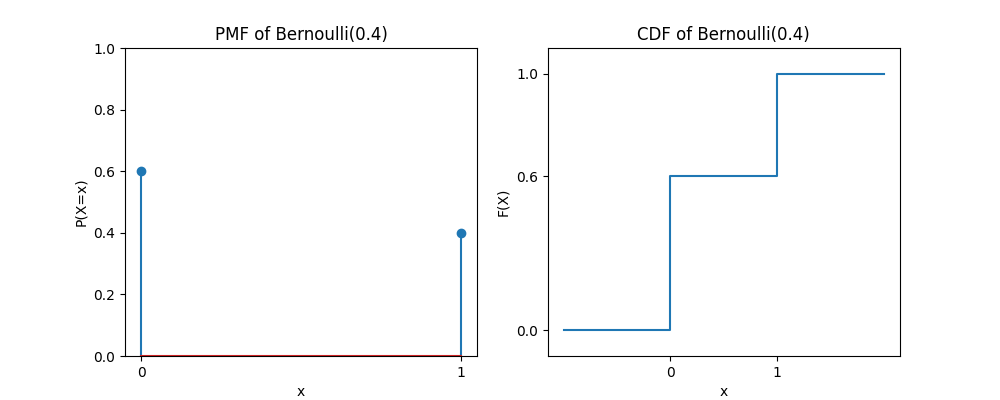
\includegraphics[width=0.9\textwidth]{figs/fig.png}
    \end{figure}
\end{frame}

\end{document}

